\part{The 6502 CPU architecture}
\frame{\partpage}

\begin{frame}{MOS Technology 6502}
	\begin{columns}
		\begin{column}{0.4\textwidth}
			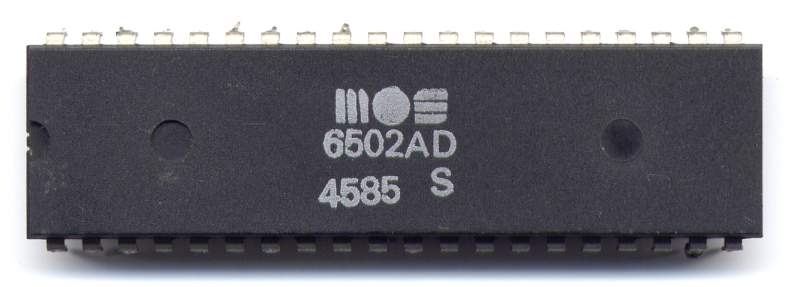
\includegraphics[width=\textwidth]{MOS_6502AD_4585_top}
		\end{column}
		\begin{column}{0.58\textwidth}
			\begin{itemize}
				\pause\item Designed by Chuck Peddle and team at \textbf{MOS Technology}
				\pause\item \textbf{8-bit} CPU, 16-bit addressing
				\pause\item Clocked between \textbf{1MHz} and \textbf{3MHz}
				\pause\item First produced in \textbf{1975}
				\pause\item Still in production \textbf{today}
			\end{itemize}
		\end{column}
	\end{columns}
\end{frame}

\begin{frame}{Uses of the 6502}
	\begin{columns}
		\begin{column}{0.32\textwidth}
			\pause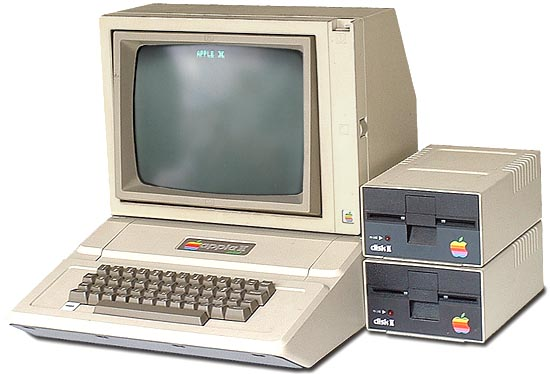
\includegraphics[width=\textwidth]{appleii}
		\end{column}
		\begin{column}{0.32\textwidth}
			\pause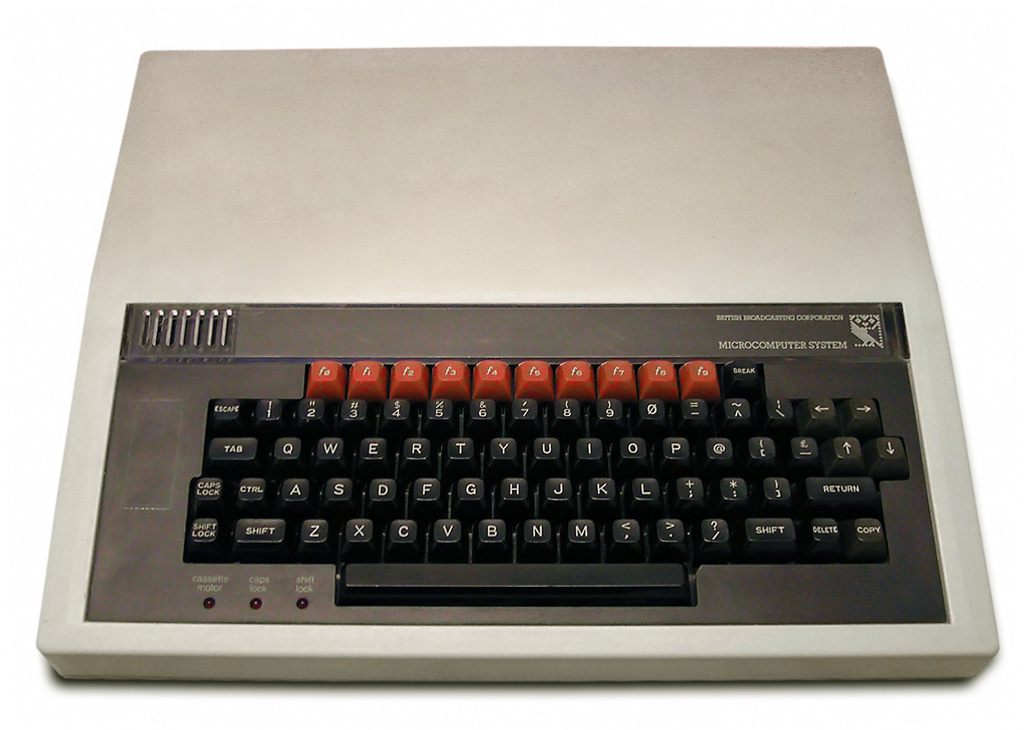
\includegraphics[width=\textwidth]{bbcmicro}
		\end{column}
		\begin{column}{0.32\textwidth}
			\pause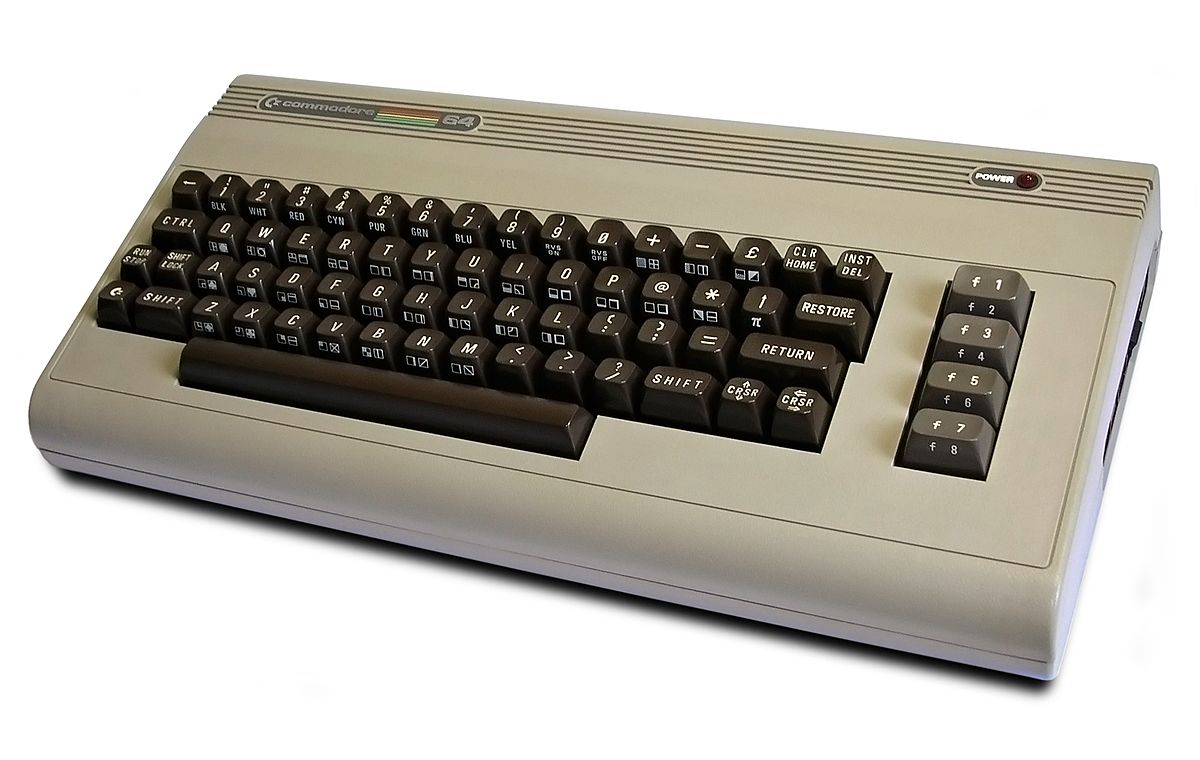
\includegraphics[width=\textwidth]{Commodore64}
		\end{column}
	\end{columns}
	\begin{columns}
		\begin{column}{0.32\textwidth}
			\pause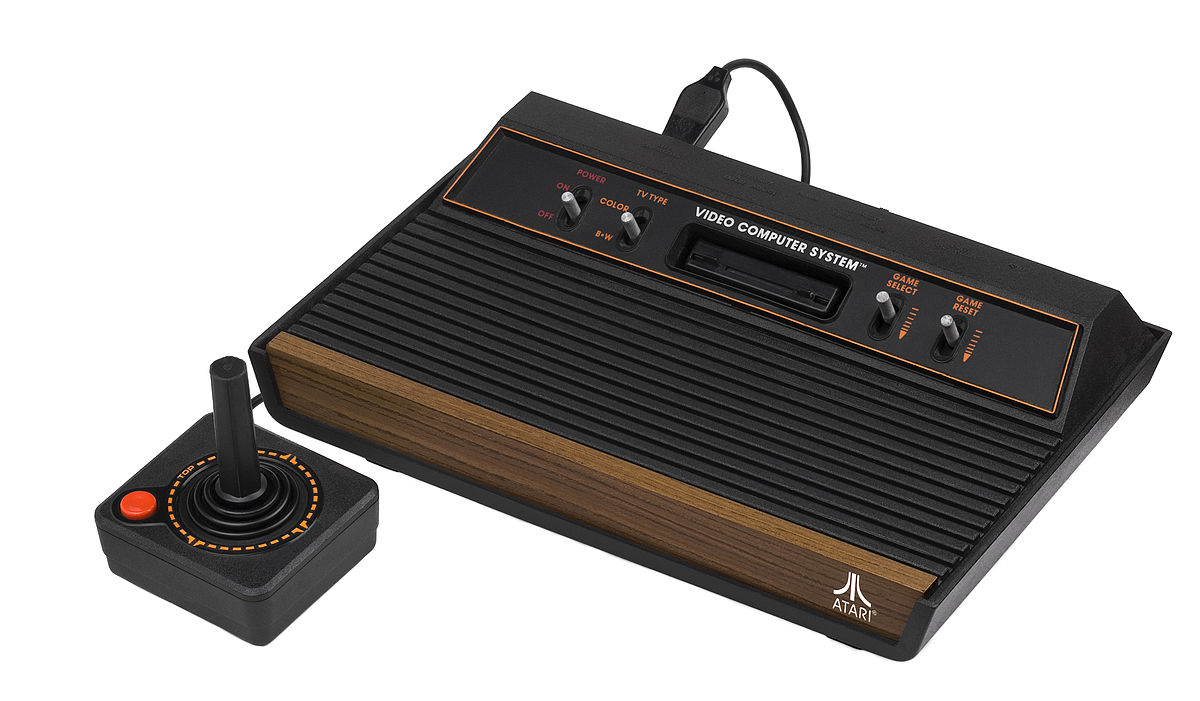
\includegraphics[width=\textwidth]{atari2600}
		\end{column}
		\begin{column}{0.32\textwidth}
			\pause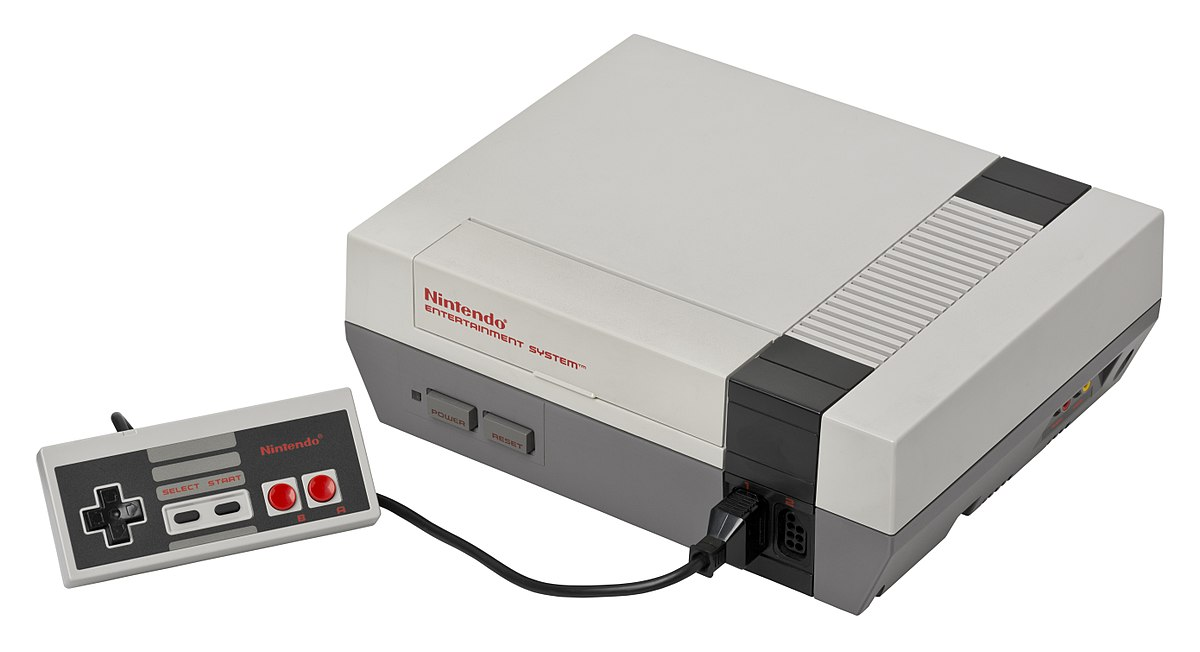
\includegraphics[width=\textwidth]{nes}
		\end{column}
		\begin{column}{0.32\textwidth}
			\pause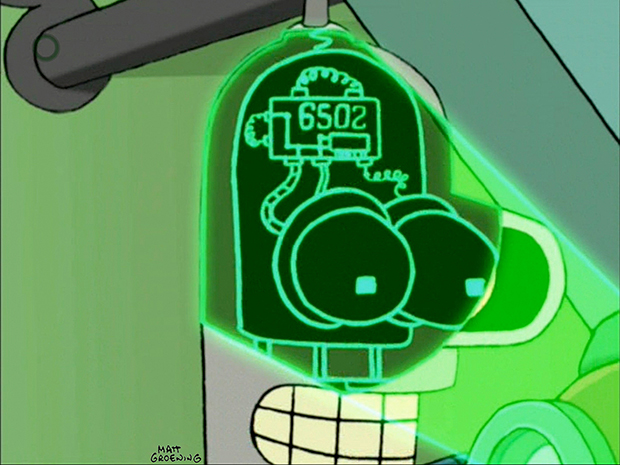
\includegraphics[width=\textwidth]{bender}
		\end{column}
	\end{columns}
\end{frame}

\begin{frame}{Recap: hexadecimal notation}
	\begin{columns}
		\begin{column}{0.32\textwidth}
			\begin{itemize}
				\pause\item We usually write numbers in \textbf{decimal} i.e.\ \textbf{base 10}
				\pause\item Hexadecimal is \textbf{base 16}
				\pause\item Uses extra digits:
					\begin{itemize}
						\item \texttt{A}=10, \texttt{B}=11, ..., \texttt{F}=15
					\end{itemize}
			\end{itemize}
		\end{column}
		\pause
		\begin{column}{0.64\textwidth}
			\begin{tabular}{rl|rl|rl}
				\textbf{Hex} & \textbf{Dec} & \textbf{Hex} & \textbf{Dec} & \textbf{Hex} & \textbf{Dec} \\
				\texttt{00} & 0             & \texttt{10} & 16            & \texttt{F0} & 240           \\
				\texttt{01} & 1             & \texttt{11} & 17            & \texttt{F1} & 241           \\
				$\vdots$ & $\vdots$         & $\vdots$ & $\vdots$         & $\vdots$ & $\vdots$         \\
				\texttt{09} & 9             & \texttt{19} & 25            & \texttt{F9} & 249           \\
				\texttt{0A} & 10            & \texttt{1A} & 26            & \texttt{FA} & 250           \\
				\texttt{0B} & 11            & \texttt{1B} & 27            & \texttt{FB} & 251           \\
				\texttt{0C} & 12            & \texttt{1C} & 28            & \texttt{FC} & 252           \\
				\texttt{0D} & 13            & \texttt{1D} & 29            & \texttt{FD} & 253           \\
				\texttt{0E} & 14            & \texttt{1E} & 30            & \texttt{FE} & 254           \\
				\texttt{0F} & 15            & \texttt{1F} & 31            & \texttt{FF} & 255           
			\end{tabular}
		\end{column}
	\end{columns}
\end{frame}

\begin{frame}{How a CPU works}
	\begin{itemize}
		\pause\item Executes a series of \textbf{instructions} stored in \textbf{memory}
		\pause\item An instruction is stored as an \textbf{opcode} followed by 0 or more \textbf{arguments}
		\pause\item CPU has several \textbf{registers}, each storing a single value
		\pause\item Instructions can read and write values in \textbf{registers} and in \textbf{memory},
			and can perform \textbf{arithmetic and logical} operations on them
		\pause\item The \textbf{program counter (PC)} register stores the address of the next instruction to execute
	\end{itemize}
\end{frame}

\begin{frame}{Registers on the 6502}
	\begin{itemize}
		\pause\item 6502 is an \textbf{8-bit} CPU, meaning each register stores \textbf{8 bits} of data
			\begin{itemize}
				\pause\item 1 byte
				\pause\item A number between 0 and 255
			\end{itemize}
		\pause\item A = \textbf{accumulator}
		\pause\item X, Y = \textbf{index} registers
		\pause\item SP = \textbf{stack pointer} register
		\pause\item PC = \textbf{program counter} register (16 bits)
		\pause\item \textbf{Status} register, composed of seven 1-bit \textbf{flags}
	\end{itemize}
\end{frame}

\begin{frame}{Assembly language}
	\begin{itemize}
		\pause\item Translates \textbf{directly} to machine code
		\pause\item I.e.\ 1 line of assembly = 1 CPU instruction
		\pause\item An \textbf{assembler} translates assembly to machine code
			\begin{itemize}
				\pause\item I.e.\ an assembler is a ``compiler'' for assembly language
			\end{itemize}
		\pause\item Each CPU architecture has its own instruction set therefore
			its own assembly language
	\end{itemize}
\end{frame}

\begin{frame}{Our first assembly program}
	\pause\lstinputlisting{01.asm}
	\pause Try it out! \url{http://skilldrick.github.io/easy6502/}
\end{frame}

\begin{frame}{Our first assembly program}
	\pause \lstinputlisting[firstline=1, lastline=1]{01.asm}
	\begin{itemize}
		\pause\item Store the value \texttt{01} (hexadecimal) into register A
		\pause\item \lstinline{LDA} (``load accumulator'') stores a value in register A
		\pause\item \lstinline{####} denotes a literal number (as opposed to a memory address)
		\pause\item \lstinline{$} denotes hexadecimal notation
		\phantom{\lstinline{$}} % fix highlighting
	\end{itemize}
\end{frame}

\begin{frame}{Our first assembly program}
	\pause \lstinputlisting[firstline=2, lastline=2]{01.asm}
	\begin{itemize}
		\pause\item Write the value of register A into memory address \texttt{0200} (hex)
		\pause\item \lstinline{STA} (``store accumulator'') copies the value of register A into main memory
		\pause\item Note that address is a \textbf{16-bit} number (2 bytes, 4 hex digits)
		\pause\item In this emulator the display is ``memory mapped'', with 1 byte per pixel, starting from address \texttt{0200}
			\begin{itemize}
				\item This may \textbf{not} be the case on other 6502-based systems!
			\end{itemize}
	\end{itemize}
\end{frame}

\begin{frame}[fragile]{Assembly to machine code}
	\begin{columns}
		\begin{column}{0.48\textwidth}
			\pause\lstinputlisting{01.asm}
		\end{column}
		\begin{column}{0.48\textwidth}
			\pause
			\begin{lstlisting}
A9 01
8D 00 02
A9 05
8D 01 02
A9 08
8D 02 02
			\end{lstlisting}
		\end{column}
	\end{columns}
	\pause Note that the 6502 is \textbf{little endian}
	\begin{itemize}
		\pause\item In 16-bit values, the ``high'' byte comes before the ``low'' byte
		\pause\item Intel x86 is also little endian
	\end{itemize}
\end{frame}

\begin{frame}[fragile]{Looping}
	\begin{itemize}
		\pause\item PC normally \textbf{advances} to the next instruction
		\pause\item Some instructions \textbf{modify} the PC
		\pause\item E.g.\ \lstinline{JMP} (jump) sets the PC to the specified address
	\end{itemize}
	\pause
	\begin{lstlisting}
INC $0200 ; add 1 to the value at address 0200
JMP $0600 ; jump back to beginning of program
	\end{lstlisting}
	\begin{itemize}
		\pause\item In this emulator the program always starts at address \texttt{0600}
			\begin{itemize}
				\item This may \textbf{not} be the case on other 6502-based systems!
			\end{itemize}
	\end{itemize}
\end{frame}

\begin{frame}[fragile]{Labels}
	\begin{itemize}
		\pause\item Don't use explicit jump locations in your code, it's not maintainable!
		\pause\item Can add a \textbf{label} to a line of code, by giving a name followed by a colon
		\pause\item Labels can then be used in instructions
	\end{itemize}
	\pause
	\begin{lstlisting}
start:
    INC $0200
    JMP start
	\end{lstlisting}
	\begin{itemize}
		\pause\item \lstinline{start} is essentially a constant with value \lstinline{$0600}
		\pause\item The assembled code is exactly the same as for the previous slide
	\end{itemize}
\end{frame}

\begin{frame}[fragile]{Conditional branching}
	\pause
	\lstinputlisting{02.asm}
	\pause
	\begin{algorithmic}
		\State $X = 8$
		\Do
			\State $X = X-1$
			\State $\operatorname{memory}[0200] = X$
		\doWhile{$X \neq 3$}
		\State $\operatorname{memory}[0201] = X$
	\end{algorithmic}
\end{frame}

\begin{frame}[fragile]{Conditional branching}
	\begin{itemize}
		\pause\item Assembly language does not have \textbf{structured programming} constructs
			such as if/else, switch/case, for, while, etc.
		\pause\item However all of these can be implemented using branch instructions
		\pause\item ... which is exactly how compilers implement them
	\end{itemize}
\end{frame}

\begin{frame}[fragile]{Subroutines}
	\begin{itemize}
		\pause\item \lstinline{JSR} (jump to subroutine) works like \lstinline{JMP}, but stores the current PC
		\pause\item \lstinline{RTS} (return from subroutine) jumps back to the instruction
			after the \lstinline{JSR}
		\pause\item These are used to implement \textbf{function calls}
	\end{itemize}
\end{frame}

\begin{frame}[fragile]{Addressing modes}
	\begin{itemize}
		\pause\item Immediate: \lstinline{LDA #$42}
			\begin{itemize}
				\pause\item Load the literal value 42 (hex) into register A
			\end{itemize}
		\pause\item Absolute: \lstinline{LDA $42}
			\begin{itemize}
				\pause\item Load the value stored at memory address 42 (hex) into register A
			\end{itemize}
		\pause\item That \lstinline{#} makes a big difference!
		\pause\item Note that these actually assemble to \textbf{different} CPU instructions
	\end{itemize}
\end{frame}

\begin{frame}[fragile]{Indexed addressing}
	\begin{lstlisting}
LDA $0200,X
	\end{lstlisting}
	\begin{itemize}
		\pause\item Look up the value stored at memory address
			$$ \texttt{0200} + (\text{value of X register}) $$
			and store it in A
		\pause\item Can also do \lstinline{LDA $0200,Y}
		\pause\item ... but \textbf{only} \lstinline{X} and \lstinline{Y} registers can be used for indexed addressing
	\end{itemize}
\end{frame}

\begin{frame}[fragile]{Indexed addressing}
	\begin{lstlisting}
  LDX #0      ; X=0
loop:
  TXA         ; A=X
  STA $0200,X ; store A to 0200+X
  INX         ; X++
  JMP loop    ; loop forever
	\end{lstlisting}
	\begin{itemize}
		\pause\item Why does it stop $\frac14$ of the way down?
		\pause\item Hint: it stops after filling 256 pixels...
	\end{itemize}
\end{frame}

\begin{frame}{Next steps}
	\begin{itemize}
		\pause\item \textbf{Work through} the tutorials on \url{http://skilldrick.github.io/easy6502/}
		\pause\item \textbf{Understand} and try to \textbf{modify} the Snake game code
	\end{itemize}
\end{frame}
